\begin{abstract}
Metaphor is far more than a literary device. It is a
fundamental cognitive ability that drives the human capacity for reasoning about
states, situations, and actions in the world~\cite{Gibbs1994,Lakoff1980}.
Metaphor---which involves understanding of abstract concepts in
terms of relatively more basic ones---permeates political
discourse~\cite{Lakoff2008,Matlock2012}. Its ubiquity in everyday discourse
is evident in the frequent use of statements such as ``It's time
to drain the swamp'', ``Obama sprinted toward victory on Election Day'', and
``Trump attacks Jeff Sessions over Russian probe methods''. No one is releasing
water. No one is running. No one is causing physical harm. How is metaphorical
violence expressed, for instance, expressions with words such as ``attack'',
``slaughter'', and ``hit'', and how does such language influence political
thought and communication? Here, we describe novel time-resolved 
observations and explanatory dynamical models of the use of metaphorical 
violence language in political discourse on U.S. cable television news in the 
period leading up to the two most recent presidential elections. 
Our results quantify the details and dynamics of the use of these metaphors, 
revealing how cable news shows act as reporters, promoters, 
expectation-setters, and ideological agents in different degrees in 
response to differing cultural situations. Our work has implications for 
shaping political discourse and influencing political attitudes. 	
\end{abstract}

\section{Introduction}

Conceptual metaphor theory holds that linguistic
metaphors, such as ``Costs are rising,'' reflect a process whereby one concept is
structured in terms of another; in this case, costs are conceptualized in terms
of physical verticality. In this way, metaphor is not just language; it is a way
of thinking~\cite{Gibbs1994,Lakoff1980,Thibodeau2011}  and it is intimately
linked to emotions \cite{Kovecses2010} and grounded in bodily
experience~\cite{Gallese2005}. Because metaphor is so pervasive and because many
people care about political matters, it is useful to consider how it is used and
how it might shape public opinion on matters of national or international
importance, such as climate change~\cite{Flusberg2017} and
politics~\cite{Lakoff2008,Lakoff2012}. 

We are especially interested in violence
metaphors in the context of political discourse. We define \emph{violence
metaphors} as those that portray political concepts in terms of physical
violence. Consider two statements from cable TV news in 2012 that both feature the
word ``attack'':
\begin{exe} \ex Because we want you to pay for your own birth control,
  that's an \emph{attack} on your womb like we're flying a predator drone over your
  fallopian tubes and calling in a strike?\footnote{Adam Carolla on \emph{The
  O'Reilly Factor}, FOX News, September 10, 2012; \url{https://goo.gl/jVBsqH}}
  \label{ex:carolla} 
  \ex John McCain and his allies have been trying to turn the
  Benghazi attacks into a political scandal for the president since
  September.\footnote{Chris Matthews on \emph{Hardball with Chris Matthews},
  MSNBC, November 15, 2012; \url{https://goo.gl/Pfs4Sc}}
\label{ex:benghazi-attacks} \end{exe} The first statement refers to political
efforts to force employers to provide insurance that covers birth control for
women.  It is metaphorical because the
womb is not physically assaulted. Here there is a mapping from a \emph{source domain} of  violence,
associated with bodily harm, wars, battles, etc., to  a \emph{target domain} of
argumentation, in this case, about who should pay for birth control. The second
refers literally to a terrorist attack in the town of Benghazi;
clearly, it is not metaphorical. 

Metaphor can heighten emotions in political
communication~\cite{Charteris-Black2009}. Reporters seem to understand this
well.  They use metaphor to draw attention and create a reaction in readers and
listeners~\cite{Lakoff2008}. Americans have long been fascinated by the
political theater afforded by television, and, over time, the media has come to
frame debates as violent events~\cite{Schroeder2008}. The trend toward increased
spectacle and competitive framing continues; 
for instance, political campaigns are often portrayed as
military campaigns (see Burnes, 2011, and Kalmoe, 2014). In the U.S. and
elsewhere, political contests are now routinely conceptualized in terms of
physical actions, often taken against another, such as footraces
(see Matlock, 2013) or battles (see Flusberg, Matlock, and Thibodeau, 2018). 
Importantly, using metaphorical violence in political discourse has 
real consequences on reasoning; for instance, it can increase the tendency to polarize
(see Kalmoe, Gubler, and Wood, 2018).

The influence and diverse range of ideological perspectives of U.S. cable
television news make it an important system to understand.  Interested in how
metaphorically violent language would vary in reportage around debates leading
up to a U.S. presidential election, we analyzed language used on the
most-watched cable television news networks MSNBC, CNN, and Fox
News~\cite{OConnell2017}. CNN and MSNBC are on the progressive end of the
ideological spectrum, and Fox News, the conservative end~\cite{Pew2014}. Right
before the 2016 presidential election, 40\% of Trump voters said Fox News was
their primary source of news, whereas 27\% of Clinton voters said theirs was 
MSNBC or CNN~\cite{Pew2017TrumpClinton}. For our analysis, we analyzed the use of metaphorical violence language on two
different shows from each of these three networks during September 1 to November 30 in 2012
and 2016, periods in which four major political events occurred: three
presidential debates and election day.

The main questions of interest concern how metaphorical violence was used leading
up to election day: Which networks produce the most
metaphorical violence language? Is this consistent across years? What is the
contribution of each show to total use?  What is the difference in how often
metaphorical violence language is used, and does this change across networks or
years? Who is conceptualized more often as attacking and being attacked by
metaphorical violence, and does this change across networks and time? In
addition to revealing details of the use of metaphorical violence language on
cable television news, informing the study of political communication and
action, our results provide data for understanding a deep question in cognitive
linguistics: to what extent and how does the cultural context influence which
metaphors are used~\cite{Gibbs1997,Kovecses2010}? 

Our main results are a series of observations about the use of metaphorical
violence language across different cultural situations and by different cultural
actors. We expected metaphors to change over time in response to, or in
anticipation of, the cultural events of the presidential debates and election
day, and on the specific actions taken and language used by the candidates
themselves. We also expected metaphor use to differ across the three networks
given their differing ideologies~\cite{Lakoff2008}, though we also expected some
similarities across networks, because of shared cultural frames \cite{Kovecses2010}. 

To address these questions, we collected data
from the Internet Archive's TV News Archive (TVNA), a curated
library containing millions of short video clips from cable television news
shows from the last decade. We collected data from the two most highly rated
news shows on each network in each of the two study years (details in
the supplement). We relied on closed caption data provided by the TVNA
to create textual transcripts of each show, and searched each transcript for
words that signal, or instantiate, the source domain of violence, the
\emph{violence signal}. We considered only phrases that use one of three
violence signals---\emph{attack}, \emph{beat}, or \emph{hit}. If a violence
signal was found in an episode of a show, a human reviewer then manually decided
whether it represented metaphorical violence based on the context, annotating
the text to identify subject, verb, and object of the phrase for all uses of
metaphorical violence.  Analyzing subject and object allowed us to determine who
was portrayed as the aggressor and who was portrayed as the victim.

\section{Methods}
\subsection{Data collection and annotation}

Data were collected from the Internet Archive's TV News Archive
(TVNA).\footnote{See \url{https://archive.org/details/tv}.} Using custom
software to access, annotate, and analyze TVNA data, we could effectively
download, review, and code hundreds of hours of news broadcasts.\footnote{Our
custom software, Metacorps, is freely available at
(REDACTED FOR ANONYMITY).} We collected data from the two
most highly rated news shows on each network in each of the two study years,
relying on closed caption data  to create textual transcripts of each show. We
searched each transcript for words that signal violence, namely, \emph{attack},
\emph{beat}, or \emph{hit}. If a violence signal was found, a human reviewer
then manually decided whether it represented metaphorical violence based on
context, annotating the text to identify subject, verb, and object of the phrase
for all uses of metaphorical violence. Annotations were stored along the
transcript, date and time, show, and network to enable later analyses.

We focused primarily on three violence signals which were far the most commonly
used metaphorically among a list of twenty violence words that we initially 
considered. Our initial list was built based on a close reading of newspapers 
and other online news, and cable news transcripts. We assume there is one 
best interpretation of whether or not a statement is metaphorical. For this reason,
we do not calculate inter-rater reliability. We have, however, made our 
full datasets available, including the original phrases found in cable news 
transcripts containing metaphorical and non-metaphorical violence, and all
our annotations (URL REDACTED FOR ANONYMITY). We provide a way to review our 
annotations, modify them, and re-run all these analysis through a Docker 
container of the Metacorps web application and a Jupyter notebook that 
runs all analyses. Instructions for reviewing our analyses and performing your
own are in the on GitHub (URL REDACTED FOR ANONYMITY).

We collected cable television news transcripts indexed by date, network, and
show. We identified and counted daily metaphorical
violence use based on the violence signals \emph{attack}, \emph{hit}, and
\emph{beat} (see Table~\ref{tab:words}). We counted the daily instances of
Democratic presidential candidates (Barack Obama in 2012 and Hillary Clinton in
2016) and Republican presidential candidates (Mitt Romney in 2012 and Donald
Trump in 2016) appearing as the aggressor or victim of metaphorical violence
(see Table~\ref{tab:subjobj}). Sometimes the aggressor and victim of metaphorical 
violence are clear, as a reporter on CNN's \emph{Anderson Cooper 360}
described Clinton criticizing Trump in the first debate as Clinton hitting Trump
\footnote{\url{https://archive.org/details/CNNW_20160928_040000_Anderson_Cooper_360/start/2820/end/2880}}:

\begin{exe}
  \ex Clinton \emph{hit} Trump for voicing support for invading Iraq and calling
    climate change a hoax.
\end{exe}
The subject and object are not always explicitly
specified in a single sentence, but often can be inferred. We include
a reference to the video link on the Internet Archive so the reader can understand
the context which leads us to our inferences.
For instance, a guest on \emph{The Rachel Maddow Show}
described some of Donald Trump's comments as a metaphorical 
\emph{attack} on Hillary Clinton, without saying their names explicitly in the sentence\footnote{\url{https://archive.org/details/MSNBCW_20161021_010000_The_Rachel_Maddow_Show/start/3000/end/3060}}

\begin{exe}
  \ex One joke after another \ldots was a political attack mildly veiled in
  humor.
\end{exe}

%%
% Table with network and violent words
%
\begin{table}[H]
  \centering

  \begin{subtable}{\linewidth}
    \centering
    \begin{tabular}{llrrrr}
\toprule
       &     & $f^{(1)}$ & $f^{(2)}$ & \emph{delta} & total uses \\
Violent Word & Network &           &           &            &            \\
\midrule
hit & MSNBC &      0.86 &      0.86 &      -0.00 &         67 \\
       & CNN &      0.54 &      0.11 &      -0.81 &         34 \\
       & Fox News &      0.57 &      0.33 &      -0.42 &         41 \\
\hline
beat & MSNBC &      1.03 &      1.64 &       0.59 &         89 \\
       & CNN &      0.66 &      0.63 &      -0.04 &         51 \\
       & Fox News &      0.83 &      0.53 &      -0.35 &         60 \\
\hline
attack & MSNBC &      1.30 &      3.14 &       1.42 &        127 \\
       & CNN &      2.07 &      0.32 &      -0.85 &        128 \\
       & Fox News &      2.08 &      2.00 &      -0.04 &        161 \\
\bottomrule
\end{tabular}

    \caption{\quad 2012}
    \label{tab:words-2012}
  \end{subtable}
  
  \vspace{.25in}

  \begin{subtable}{\linewidth}
    \centering
    \begin{tabular}{llrrrr}
\toprule
       &     & $f^{(1)}$ & $f^{(2)}$ & \emph{delta} & total uses \\
Violent Word & Network &           &           &            &            \\
\midrule
hit & MSNBC &      0.16 &      0.06 &      -0.63 &         10 \\
       & CNN &      0.27 &      0.45 &       0.64 &         25 \\
       & Fox News &      0.46 &      1.36 &       1.97 &         56 \\
\hline
beat & MSNBC &      0.54 &      1.47 &       1.75 &         55 \\
       & CNN &      0.50 &      0.79 &       0.59 &         45 \\
       & Fox News &      0.48 &      0.88 &       0.84 &         45 \\
\hline
attack & MSNBC &      0.61 &      1.59 &       1.62 &         61 \\
       & CNN &      1.16 &      2.59 &       1.23 &        126 \\
       & Fox News &      1.08 &      4.32 &       2.99 &        160 \\
\bottomrule
\end{tabular}

    \caption{\quad 2016}
    \label{tab:words-2016}
  \end{subtable}

  \caption{Uses and \emph{delta} for violence signals on each network in 2012 and 2016.}
  \label{tab:words}
\end{table}

\subsection{Dynamical statistical model}

We modeled change in frequency of metaphorical language use as an impulse
function with two states:

\begin{equation} \label{eq:model} 
  f[t] = \begin{cases} f^{(1)} \text{ if } t \in T^{(1)} \\
f^{(2)} \text{ if } t \in T^{(2)} 
  \end{cases} 
\end{equation}
\noindent

Many more complicated models for change in frequency are possible. Here, we
simply used the simplest model of change---that there is one state and then at
some point later there is another.  Of course, in general there many be fewer
than two states or more than two states, and there is no reason to suppose there
would be exactly two.  Nevertheless, we have opted to use the simplest possible
model, supposing there is change.

The dates for which we have data form a time series, $T$, of frequencies of use
for each of the three networks in each of the two election years, six total. All
shows do not air episodes every day. When neither of a network's two shows aired
an episode on a given day, that day is not included in $T$. On a day that is
included in $T$, there may be one or two episodes, so when considering dynamics,
we plot and model the frequency of metaphorical violence use per episode.
Frequency is simply the number of uses in a day divided by the number of
episodes of the shows in that day. The time series are modeled as beginning at a
mean frequency $f^{(1)}$ (State 1), then at some point later, the mean frequency
changes to $f^{(2)}$ (State 2). Model fitting amounts to categorizing dates as
either belonging to State 1 or State 2. These are subsets of $T$, with the State
1's dates denoted $T^{(1)}$ and State 2's dates denoted $T^{(2)}$:

\[ T^{(2)} = \{t \in T: t_{first}^{(2)} \leq t \leq t_{last}^{(2)} \} \]
\noindent and 

\[ T^{(1)} = T~\setminus~T^{(2)}.  \] \noindent To fit parameters
$t_{first}^{(2)}$ and $t_{last}^{(2)}$ to the model to minimize error, we used
Bayesian multi-model inference, which allowed us to quantify the likelihood that
alternate parameterizations would better fit the observed
data~\cite{Burnham2011}. Specifically, to determine the best-fitting model, we
use Bayesian multimodel inference to infer which parameters are most likely to
best represent the system dynamics \cite{Burnham2011}.  Choosing a model with
minimum AIC when all models have the same number of parameters is equivalent to
selecting the model with minimum error, or maximum log-likelihood. Using the AIC
allows us to calculate the relative likelihood of different parameterizations.
Once the minimum AIC is found, call it $\text{AIC}_{min}$, the relative
likelihood that model parameterization $i$ outperforms the model with minimum
AIC is $\text{exp}(\frac{\text{AIC}_{min} - \text{AIC}_i}{2})$. The AIC on
its own tells us nothing about how well the model matches the data, only  how
well the model performs relative to other models. An added feature of using this
inference approach is that it reveals more about the system dynamics than if we
were to simply select and use the  model that minimized error. It also provides
a foundation for future work that considers more complex metaphorical violence
language dynamics. 

Given a model we can calculate the fractional change in frequency, which we
denote by \emph{delta}: 
\begin{equation} 
  delta = \frac{f^{(2)} - f^{(1)}}{f^{(1)}}.  
  % \text{\emph{delta}} = \frac{f^{(2)} - f^{(1)}}{f^{(1)}}.  
  \label{eq:delta} 
\end{equation} 
\noindent \emph{Delta},
$t^{(2)}_{first}$, and $t^{(2)}_{last}$ enable us to compare changes in
metaphorical violence language frequency across the networks and over time.


\section{Analysis}

Overall, we observed 758 uses of metaphorical violence language in 2012, and 583
in 2016. In 2012, the MSNBC show \emph{Hardball} alone contained 208
metaphorical violence uses, whereas other MSNBC shows ranged from 60 to 120.
Shows on CNN were more consistent, ranging from 99 to 118, as were shows on Fox
News, ranging from 130 to 150. The distribution of specific violence signals
across networks and shows was similar in both 2012 and 2016: \emph{attack} was
used most, \emph{beat} next most, and \emph{hit} least. Interestingly, in 2012
MSNBC led in total metaphorical violence language use, and \emph{hit} and
\emph{beat} were used more often than \emph{attack} on that network.
In both 2012 and 2016, the
Republican candidate was both the aggressor and victim of metaphorical violence
more often than the Democratic candidate. In 2016, Trump was characterized as
doing metaphorical violence 102 times by Fox News, compared to 30 times for
Clinton. This finding is consistent with other research that suggests
conservatives more often conceptualize interpersonal relationships in terms of
violence or are more likely to resort to violence in interpersonal relationships
than progressives~\cite{Lakoff1996, Cohen1996}. 

To compare the dynamics and time-course of metaphorical violence use across the
different networks, we modeled change in frequency of use as an impulse function
with two states (Equation 1). We fit our dynamical
model for six time series, one for each network in each study year. Bayesian
multi-model inference allowed us to identify the best-fit model and to quantify
the relative likelihood of other parameterizations being better (all best-fits were
significant). We next calculated change in relative frequency of metaphorical
violence use, or \emph{delta}, across networks, violence signals, and clausal
subject and object (Equation 2). We found both positive and negative values for \emph{delta},
meaning that metaphorical violence language did not increase uniformly within
the study period across networks and years. Fox News and CNN had negative
\emph{deltas} in 2012. In the case of Fox News in 2012, metaphorical violence
language decreased starting September 9 and ending September 25, the days
leading up to the first presidential debate on October 3. CNN's use dipped after
November 6, election day. In 2012, MSNBC was the only network with a positive
change, starting on September 13 and ending September 27, just before the first
debate. In 2016, \emph{delta} was positive and larger in magnitude for all three
networks, with the start date of the elevated state overlapping to a much
greater degree (see Figure~\ref{fig:ModelFits}). This reflects the differences in cable news
viewership between 2012 and 2016: 67.2 million watched the first
Obama-Romney debate in 2012 compared with 84 million for the first Clinton-Trump
debate in 2016 \cite{Perlberg2016}.  Part of this broad, synchronized excitement about 
the election 	may have been because of the big personalities of the two main contenders: 
Clinton was the first woman candidate and a controversial
first-lady.  Candidate Trump was a rich, controversial television star.

\begin{figure}[H]
  \vspace{.2in}
  \centering
  \begin{subfigure}{0.7\linewidth}
    \centering
    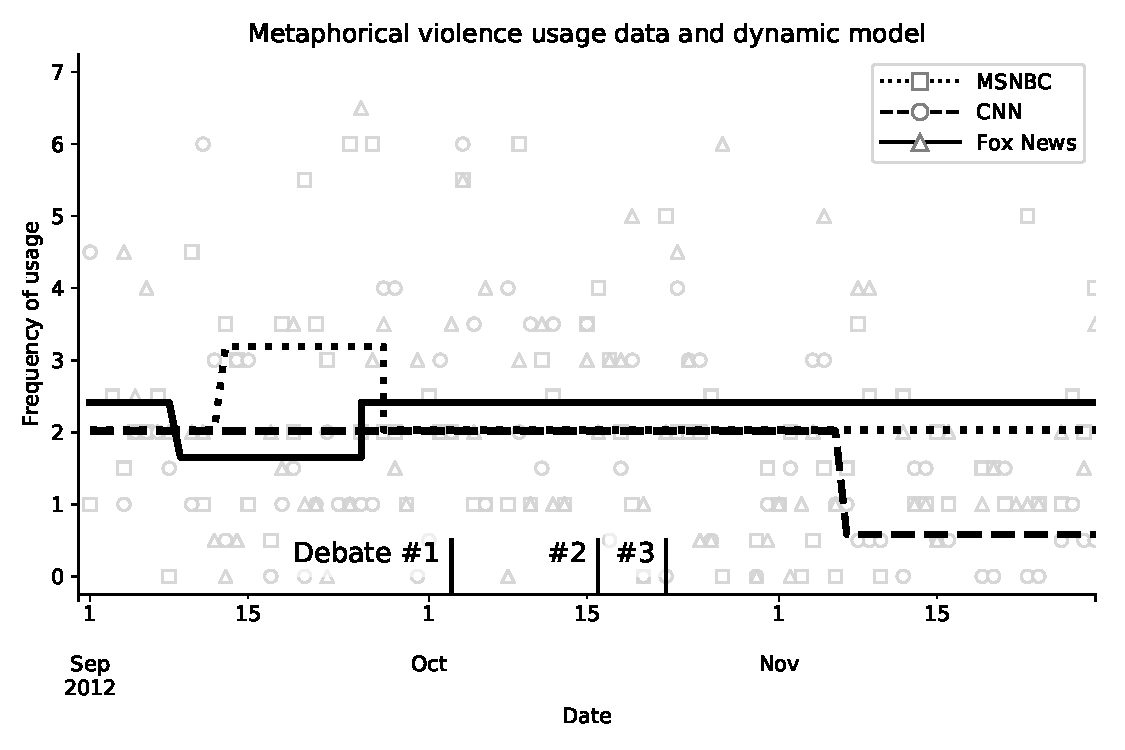
\includegraphics[width=\textwidth]{Figures/ModelFits-2012.pdf}
   \caption{\quad2012}
    \label{fig:ModelFits-2012}
  \end{subfigure}
  \begin{subfigure}{0.7\linewidth}
    \centering
    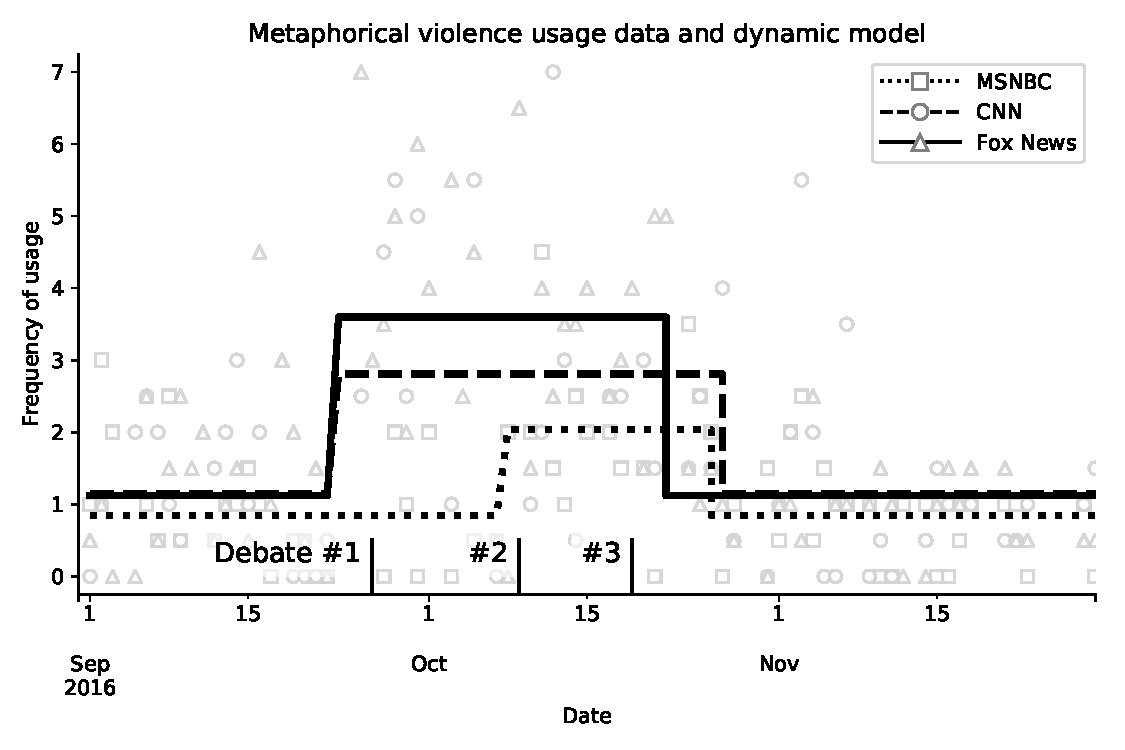
\includegraphics[width=\textwidth]{Figures/ModelFits-2016.pdf}
   \caption{\quad2016}
    \label{fig:ModelFits-2016}
  \end{subfigure}

  \caption{Observed daily frequencies (markers) and best-fit models (lines).
    The dynamical impulse model is given in 
    Equation 1. In four of the six network-year pairs, 
    there is an increase in the frequency of metaphorical violence language in the
    three-month study period: MSNBC in 2012 and all three networks in 2016. 
    However, two of the six network-year pairs showed decreases in frequency
    of metaphorical violence language use in one three-month period: CNN and Fox News
    in 2012. 
  } 
  \label{fig:ModelFits}
\end{figure}

MSNBC's positive \emph{delta} in 2012 resulted mainly
from an increased use of the signal \emph{attack}. There was no change in use of
the signal \emph{hit} on MSNBC. CNN's use of \emph{hit} and \emph{attack}
decreased by about 80\%. On Fox News in 2012, most of the decrease in overall
metaphorical violence use resulted from decreases in the use of \emph{hit} and
\emph{beat}, with \emph{attack} use remaining nearly constant. In 2016,
\emph{deltas} were positive for all networks. All \emph{deltas} were positive
for violence signals as well, with one exception: MSNBC's use of \emph{hit} fell
by 63\%. MSNBC's use of \emph{beat} and \emph{hit} increased by a factor of
almost 2. In 2016, CNN's use of \emph{attack} accounted for most of its overall
increase in metaphorical violence language use, and for Fox News, use of
\emph{attack} increased by nearly 300\%. 

\begin{table}
  \centering
  \bgroup
    \begin{subtable}{\textwidth}
      \centering
      \begin{tabular}{lr}
        \toprule
        Show (Network) & Total Uses \\
        \midrule
        The Rachel Maddow Show (MSNBC) & 93 \\
        Hardball With Chris Matthews (MSNBC) & 208 \\
        Anderson Cooper 360 (CNN) & 99 \\
        Piers Morgan Tonight (CNN) & 118 \\
        The O'Reilly Factor (Fox News) & 141 \\
        Hannity (Fox News) & 133 \\
        \bottomrule
      \end{tabular}
      \caption{Total number of uses metaphorical violence language by news show in 2012}
      \label{tab:by-show-2012}
    \end{subtable} \\  \vspace{1.5em}
    \begin{subtable}{\textwidth}
      \centering
      \begin{tabular}{lr}
        \toprule
        Show (Network) & Total Uses \\
        \midrule
        The Rachel Maddow Show (MSNBC) & 66 \\
        The Last Word with Lawrence O'Donnel (MSNBC) & 80 \\
        Anderson Cooper 360 (CNN) & 100 \\
        Erin Burnett OutFront (CNN) & 118 \\
        The O'Reilly Factor (Fox News) & 146 \\
        The Kelly File (Fox News) & 148 \\
        \bottomrule
      \end{tabular} \quad
      \caption{Total number of uses metaphorical violence language by news show in 2016}
      \label{tab:by-show-2016}
    \end{subtable}
  \egroup
  \caption{Total uses by show in each of the two study years}
  \label{tab:by-show}
\end{table}

In 2012, the candidates were involved in less of the metaphorical violence than
in 2016 (Table \ref{tab:subjobj}). Two of the three networks showed a decrease in overall metaphorical
violence use at some point in the three-month study period in 2012. Even the
increase in use on MSNBC was not as pronounced in 2012 as it was in 2016, with a
\emph{delta} of  0.57 in 2012 and 1.40 in 2016. Changes in frequency of
metaphorical violence language use were uniformly positive and larger in
magnitude in 2016, beginning before the first presidential debate (September 26)
and ending soon after the last debate (October 19). CNN and Fox News showed
increased frequency on the same day, September 9, decreasing a few days apart,
October 27 for CNN and October 22 for Fox News. MSNBC's frequency of the use of
metaphorical violence language rose later, on October 8, but decreased around
the same time as the other networks, on October 26. 

\begin{table}[!h]
  \vspace{.25in}
  \centering
  \begin{subtable}{\linewidth}
    \centering
    \begin{tabular}{llrrrr}
\toprule
                    &     & $f^{(1)}$ & $f^{(2)}$ & \emph{delta} & total uses \\
Subject/Object & Network &           &           &            &            \\
\midrule
Subject=Barack Obama & MSNBC &      0.49 &      0.38 &      -0.05 &         27 \\
                    & CNN &      0.58 &      0.12 &      -0.23 &         30 \\
                    & Fox News &      0.55 &      0.50 &      -0.02 &         31 \\
\hline
Subject=Mitt Romney & MSNBC &      0.51 &      0.77 &       0.13 &         33 \\
                    & CNN &      0.72 &      0.00 &      -0.36 &         36 \\
                    & Fox News &      0.52 &      0.57 &       0.02 &         31 \\
\hline
Object=Barack Obama & MSNBC &      0.65 &      0.69 &       0.02 &         41 \\
                    & CNN &      0.74 &      0.00 &      -0.37 &         39 \\
                    & Fox News &      0.54 &      0.50 &      -0.02 &         33 \\
\hline
Object=Mitt Romney & MSNBC &      0.63 &      0.77 &       0.07 &         41 \\
                    & CNN &      0.81 &      0.11 &      -0.35 &         44 \\
                    & Fox News &      0.83 &      0.79 &      -0.02 &         51 \\
\bottomrule
\end{tabular}

    % \begin{tabular}{lclrrrr}
\toprule
                 &   &     & $f^{(1)}$ & $f^{(2)}$ & reactivity & total uses \\
  Subject/Object & total uses & Network &           &           &            &            \\
\midrule
  Subject=Barack Obama & 88 &MSNBC &      0.49 &      0.38 &      -0.21 &         27 \\
                     & & CNN &      0.58 &      0.12 &      -0.78 &         30 \\
                     & & Fox News &      0.55 &      0.50 &      -0.08 &         31 \\
\hline
  Subject=Mitt Romney& 100 & MSNBC &      0.51 &      0.77 &       0.51 &         33 \\
                     & & CNN &      0.72 &      0.00 &      -1.00 &         36 \\
                     & & Fox News &      0.52 &      0.57 &       0.09 &         31 \\
\hline
  Object=Barack Obama&113 & MSNBC &      0.65 &      0.69 &       0.06 &         41 \\
                     & & CNN &      0.74 &      0.00 &      -1.00 &         39 \\
                     & & Fox News &      0.54 &      0.50 &      -0.08 &         33 \\
\hline
  Object=Mitt Romney& 136& MSNBC &      0.63 &      0.77 &       0.22 &         41 \\
                    &  & CNN &      0.81 &      0.11 &      -0.86 &         44 \\
                    &  & Fox News &      0.83 &      0.79 &      -0.06 &         51 \\
\bottomrule
\end{tabular}

    \caption{\quad 2012}
    \label{tab:subjobj-2012}
  \end{subtable}
  
  \vspace{.25in}

  \begin{subtable}{\linewidth}
    \centering
    \begin{tabular}{llrrrr}
\toprule
                    &     & $f^{(1)}$ & $f^{(2)}$ & \emph{delta} & total uses \\
Subject/Object & Network &           &           &            &            \\
\midrule
Subject=Hillary Clinton & MSNBC &      0.25 &      0.18 &      -0.04 &         15 \\
                    & CNN &      0.39 &      0.52 &       0.06 &         29 \\
                    & Fox News &      0.25 &      0.80 &       0.28 &         30 \\
\hline
Subject=Donald Trump & MSNBC &      0.44 &      1.35 &       0.46 &         44 \\
                    & CNN &      0.81 &      1.97 &       0.58 &         86 \\
                    & Fox News &      0.75 &      2.88 &       1.06 &        102 \\
\hline
Object=Hillary Clinton & MSNBC &      0.21 &      0.41 &       0.10 &         17 \\
                    & CNN &      0.33 &      0.83 &       0.25 &         36 \\
                    & Fox News &      0.42 &      1.48 &       0.53 &         54 \\
\hline
Object=Donald Trump & MSNBC &      0.25 &      0.47 &       0.11 &         20 \\
                    & CNN &      0.58 &      0.79 &       0.10 &         44 \\
                    & Fox News &      0.70 &      1.44 &       0.37 &         64 \\
\bottomrule
\end{tabular}

    % \begin{tabular}{llrrrr}
\toprule
                    &     & $f^{(1)}$ & $f^{(2)}$ & \emph{delta} & total uses \\
Subject/Object & Network &           &           &            &            \\
\midrule
Subject=Hillary Clinton & MSNBC &      0.25 &      0.18 &      -0.04 &         15 \\
                    & CNN &      0.39 &      0.52 &       0.06 &         29 \\
                    & Fox News &      0.25 &      0.80 &       0.28 &         30 \\
\hline
Subject=Donald Trump & MSNBC &      0.44 &      1.35 &       0.46 &         44 \\
                    & CNN &      0.81 &      1.97 &       0.58 &         86 \\
                    & Fox News &      0.75 &      2.88 &       1.06 &        102 \\
\hline
Object=Hillary Clinton & MSNBC &      0.21 &      0.41 &       0.10 &         17 \\
                    & CNN &      0.33 &      0.83 &       0.25 &         36 \\
                    & Fox News &      0.42 &      1.48 &       0.53 &         54 \\
\hline
Object=Donald Trump & MSNBC &      0.25 &      0.47 &       0.11 &         20 \\
                    & CNN &      0.58 &      0.79 &       0.10 &         44 \\
                    & Fox News &      0.70 &      1.44 &       0.37 &         64 \\
\bottomrule
\end{tabular}

    \caption{\quad 2016}
    \label{tab:subjobj-2016}
  \end{subtable}

  \caption{Uses and \emph{delta} for Republican and Democratic candidates as
  subject and object of metaphorical violence.}
  \label{tab:subjobj}
\end{table}


\section{Discussion}

What might have caused the difference in timing and magnitude of changes in
the level of metaphorical violence usage between 2012 and 2016? Fox News' 
decrease in metaphorical violence usage preceding the first debate seems to
fit with the traditional role of lowering passions and expectations, and 
casting one's preferred candidate as the underdog \cite{Schroeder2008}. 
This explanation is supported by the content of the metaphors themselves. For example, on
the September 17 episode of \emph{Hannity}, Sean Hannity said, 
\begin{exe}
  \ex I want to see Romney {\em hit} harder. I want to see him \ldots take it right to (Obama).
\end{exe}
A panelist followed up, telling Hannity, ``If Romney had your passion, if
Romney had your intelligence, he would have a shot.''\footnote{https://goo.gl/mc8aXk}
Then the next day, a contributor on \emph{The O'Reilly Factor} said,
\begin{exe}
  \ex Romney is not projecting strength. He put out a statement, he got {\em attacked}, 
   and he crawled into a hole. He should have kept moving forward with what he was saying.\footnote{https://goo.gl/HJ6BWu} 
\end{exe}
The underdog strategy worked: Romney enjoyed a boost in the polls
after the first debate. Before the debate, only 29\% of survey respondents
expected Romney would ``do a better job'' in the debate. After the debate,
72\% of those who watched it thought Romney did a better job \cite{Pew2012}.

The increase in MSNBC's usage of metaphorical violence began September
13 and continued for two weeks in response to a statement made
by Mitt Romney when he was criticizing the Obama administration's response to terrorist 
attacks on a U.S. compound in Benghazi, Libya. 
Romney called the administration's response ``disgraceful'' and 
claimed they ``sympathize with those who waged the attacks.''
On September 13, Rachel Maddow described this statement as both ``\emph{attacking}''
President Obama and 
\begin{exe}
  \ex {\em attacking} U.S. diplomatic personnel in the places that were
being attacked.\footnote{\url{https://goo.gl/QD2SFv}} 
\end{exe}
Maddow went on to quote a 
``senior republican foreign policy adviser'' who said the Romney campaign was
``just trying to score a cheap news cycle \emph{hit} based on the embassy statement
and now it's just completely blown up.'' On the same day, Chris Matthews
wondered on \emph{Hardball}, 
\begin{exe}
  \ex who is pushing that and saying, `release the
statement, \emph{attack, attack, attack}'?\footnote{\url{https://goo.gl/DQULSG}} 
\end{exe}

Later on MSNBC,
Rachel Maddow covered the controversial Massachusetts
senate race between Republican Scott Brown and Democrat Elizabeth Warren. 
Maddow cast Warren, the Democrat, as the victim of metaphorical attacks. 
The controversy began in the first debate when Brown noted 
that Warren identified herself as a 
Native American on school applications, but, Brown said, ``You can see that she's not''\footnote{\url{https://www.c-span.org/video/?c4722477/attack-referred-msnbc}}. 
Maddow first addressed this event in an interview with Rep. Barney 
Frank (D-Massachusetts), when she asked him his thoughts about 
\begin{exe}
  \ex personal \emph{attacks} by Senator Brown against Elizabeth Warren.
\end{exe}
Frank said it was a 
\begin{exe}
  \ex silly \emph{attack} on the fact that she once said she was of Native American 
  ancestry\footnote{\url{https://archive.org/details/MSNBCW_20120921_040000_The_Rachel_Maddow_Show/start/2400/end/2460}}.
\end{exe}
%The \emph{attack} was not too silly for Maddow to continue to cover using
%metaphorical violence. 
Over the next seven days, Maddow or a Maddow guest used metaphorical
violence twelve times to describe Brown's comments on Warren's race at the 
debate. 

As described, 2016 differed from 2012 in quantity and
dynamics of use of metaphorical violence on cable television news. 
We now consider specific examples of metaphor use in
2016.  Donald Trump made aggression an explicit character
feature early on in the primary election campaign, 
claiming in January 2016, ``I could stand in the middle of Fifth Avenue
and shoot somebody and I wouldn't lose any voters, OK?''\footnote{\url{https://www.realclearpolitics.com/video/2016/01/23/trump_i_could_stand_in_the_middle_of_fifth_avenue_and_shoot_somebody_and_i_wouldnt_lose_any_voters.html}}
Many of Trump's statements against others either originated on Twitter 
or were echoed on Twitter. These statements were reported in 
cable news as metaphorical violence. 
Below we first give some examples demonstrating the themes of metaphorical
violence usage that made up the higher use for the three cable 
news channels we studied. As tweeting seemed to show up
regularly in 2016, we end by calculating models relating
metaphorical violence frequency to candidate tweeting.

In playing its role as cheerleaders and expectation-setters, 
CNN and Fox News anticipated a first debate where much metaphorical violence
would be done by each candidate. This anticipation partly caused increased 
metaphorical violence usage.
Fox News and CNN increased metaphorical violence usage on 
September 24 and September 25, respectively, just before the first 
presidential debate on September 26. 
It seems news outlets were expecting debates that resembled violence, not
taking the underdog strategy for either candidate as in 2012.
Both CNN and Fox News noted the novelty of having a debate between 
candidates of different genders, and the new experience for Trump of debating
a woman ``of his same generation.''
On \emph{Anderson Cooper 360} on CNN, various commenters said the 
following\footnote{\url{https://archive.org/details/CNNW_20160926_000000_Anderson_Cooper_360}}

\begin{exe}
  \ex Is he going to \emph{hit} back if \emph{attacked} tomorrow, or even if not \emph{attacked}?
  \ex There's a gender dynamic going on here.  It'll be interesting to see 
    whether he \emph{attacks} her the way he \emph{attacked} ``Little'' Marco 
    (Rubio).
  \ex (Trump) thrives on the \emph{attack} \ldots how that will work out when 
    it's a woman of his same generation \ldots that will be dramatic.
\end{exe}

The same broadcast mentions a Trump tweet that referenced Gennifer Flowers'
affair with Bill Clinton\footnote{\url{https://archive.org/details/CNNW_20160926_000000_Anderson_Cooper_360/start/120/end/180}}. A commentator goes on to quote
Jane Goodall, who said ``Trump debates like a chimp in a dominance ritual.''
Cooper's guest explained that Trump ``is not just arguing, but intimidating'' his 
opponents\footnote{\url{https://archive.org/details/CNNW_20160926_000000_Anderson_Cooper_360/start/3180/end/3240}}.''
On Fox news, September 25, host Megyn Kelly and guests on \emph{The Kelly File} 
weighed in on debate 
strategy\footnote{\url{https://archive.org/details/FOXNEWSW_20160926_010000_The_Kelly_File}}:
\begin{exe}
  \ex You have a column out saying she should get in his face and stay in his
    face \ldots put him in the pain locker and shake it around.
    You think she should \emph{attack, attack, and attack} some more. Doesn't she
    have to worry about people saying \ldots sexist terms like she is a shrew, 
    she's shrill?
  \ex What she needs to do is \emph{attack} him on many points calmly one after
    another.
  \ex If I was Donald Trump I would really stay away from \emph{attacking} Hillary
    Clinton.
\end{exe}
During a man-on-the-street segment on \emph{The O'Reilly Factor}, one 
passerby said Clinton ``\emph{beat} the [bleep] out of Donald Trump. It was
like a boxing match, Hillary hit him 1, 2, bing bing.''\footnote{\url{https://archive.org/details/FOXNEWSW_20160928_030000_The_OReilly_Factor/start/2940/end/3000}} 

In the closing minutes of the first 2016 debate, Hillary Clinton introduced the 
story of former Miss Universe
Alicia Machado. Machado won Miss Universe when Trump owned the competition
in 1996. Clinton said Trump called Machado ``Miss Piggy'' because
of Machado gained too much weight and ``Miss Housekeeping'' 
because Machado was born in Venezuela. 
This controversy reverberated throughout the rest of the presidential race.
Trump spoke out on the Fox News morning show Fox and Friends the 
next morning, and on Twitter over the 
next few days, to defend his negative view of Machado. A reporter on 
\emph{Anderson Cooper 360} cast Clinton's strategy as metaphorical violence 
on September 27
\begin{exe}
  \ex The Clinton campaign had an ad ready to \emph{hit} Trump\footnote{\url{https://archive.org/details/CNNW_20160928_040000_Anderson_Cooper_360/start/1800/end/1860}}.
\end{exe}
On the morning of September 30, in the third of
a series of three tweets about Machado, Trump called 
Machado ``disgusting'' and told readers to ``check out sex tape.''\footnote{\url{https://twitter.com/realdonaldtrump/status/781788223055994880}} 
The following quotes from the September 30 episode
of \emph{Erin Burnett OutFront}\footnote{\url{https://archive.org/details/CNNW_20160930_230000_Erin_Burnett_OutFront}} 
demonstrate how metaphorical violence was used
to describe the exchange of words on this issue, and the candidates' 
reactions and counter-reactions:

\begin{exe}
  \ex Did the debate hurt Donald Trump and are his \emph{attacks} on a former
    Miss Universe taking a toll?
  \ex In a statement (Machado) says Trump's latest \emph{attacks} are cheap lies 
    with bad intentions.
  \ex Trump is also \emph{attacking} the media.
  \ex Tonight Hillary Clinton hammering Donald Trump for his \emph{attacks} on 
    former Miss Universe Alicia Machado.
\end{exe}
Regarding Trump's tweets, Clinton herself asked at a campaign rally, ``Who
gets up at three o'clock in the morning to engage in a Twitter \emph{attack} against
a former Miss Universe?''\footnote{\url{https://archive.org/details/CNNW_20160930_230000_Erin_Burnett_OutFront/start/1020/end/1080}} 


Two days before the second debate, October 7, the Washington Post published a video
in which Trump brags that being famous enables him to 
sexually assault women\footnote{\url{https://goo.gl/tk3ZNf}}. 
Trump apologized for those words in a video posted to Twitter that night
\footnote{\url{https://twitter.com/realDonaldTrump/status/784609194234306560}} 
Along with the apology in the same video, Trump accused, ``Bill Clinton has actually
abused women, and Hillary has bullied, attacked, shamed, and 
intimidated his victims,'' and
foreshadowed ``we will discuss this more in the coming days. See you at the
debate on Sunday.'' 
Two quotes from a special edition of \emph{Last Word} illustrate the coverage
of this threat using metaphorical violence\footnote{\url{https://archive.org/details/MSNBCW_20161008_100000_The_Rachel_Maddow_Show}; although the show
ID says it's \emph{The Rachel Maddow Show}, but it is in fact 
\emph{The Last Word with Lawrence O'Donnell}}. This is also further evidence that
cable news uses metaphorical violence in their coverage of debate preparation
and in expectation-setting.  

\begin{exe}
  \ex Clinton \ldots has already been practicing for these \emph{attacks} from 
    Donald Trump \ldots she already has her playbook.
  \ex (Clinton's) team has been preparing for Donald Trump to throw every 
    possible \emph{attack} at her.
\end{exe}

% David Axelrod, as a guest on the October 14 episode of
% \emph{Anderson Cooper 360}, explained
% Trump's strategy using metaphorical violence:

% \begin{exe}
%   \ex What he's employing now is a deny and 
%     \emph{attack} strategy \ldots He's going to \emph{attack} 
%     hillary clinton as hard and as fiercely as he can, hoping to 
%     drag her numbers down, drive people to the third party, 
%     depress her turnout, and make his 41 or 42\% stand up.
% \end{exe}

On October 9, the day of the second presidential debate, 
all three channels were in an elevated state of 
metaphorical violence usage. In pre-debate coverage on \emph{The O'Reilly Factor},
Fox News anchor Tucker Carlson used metaphorical violence to 
describe his understanding of Trump's strategy
\begin{exe}
  \ex (Donald Trump) has decided not simply to \emph{attack} Hillary Clinton \ldots but to 
  \emph{attack} basically the entire American establishment, the press \ldots and
  basically the keepers of American standards.
\end{exe}
Here Donald Trump is framed as a herculean aggressor,
with the specific victims of his attacks being Clinton, the American establishment,
the press, and those who value prototypical American norms of behavior. 

% October 9 debate: ``In a notable exchange that was rehashed often 
%     on cable news...'' Trump attacked on the Benghazi issue as a counterattack
%     against Clinton's criticism that Trump was up at 3AM tweeting about 
%     Ms. Universe. \footnote{\url{https://archive.org/details/FOXNEWSW_20161010_030000_The_Kelly_File}}

% October 10: Hillary says ``Donald Trump spent his time last night
%     attacking me when he should have been apologizing.'' But even his 
%     apologies don't appear to be real apologies, at least according to 
%     Fox News. Another instance in explaining 
%     this\footnote{\url{https://archive.org/details/FOXNEWSW_20161010_000000_The_OReilly_Factor}}


On October 10, the day after the second debate, Donald Trump began criticizing Paul 
Ryan, the Speaker of the House, on Twitter. Trump 
wrote, ``Paul Ryan should spend more time on balancing the budget, jobs and 
illegal immigration and not waste his time on fighting the Republican nominee.''
Ryan had said he was ``sickened'' by Trump's comments and decided to cancel a
scheduled joint appearance with Trump \cite{Fahrentold2016}.
Trump would criticize the Speaker five more times in
the next six days on Twitter\footnote{\url{https://www.thetrumparchive.com/?searchbox=%22Paul+Ryan%22&dates=%5B%222016-07-31%22%2C%222016-11-30%22%5D}}.
All three networks reported on this exchange using metaphorical
violence. Juan Williams said this on October 15 on \emph{The O'Reilly Factor}\footnote{\url{https://archive.org/details/FOXNEWSW_20161016_030000_The_OReilly_Factor/start/420/end/480}}:

\begin{exe}
  \ex That is something that Donald Trump is spending time on, attacking Paul
  Ryan because Paul Ryan is distancing himself, but he's attacking a fellow
  Republican instead of broadening or shoring up his base with republicans.
\end{exe}
In the following weeks, there were many more contentous issues which caused a
series of ``attacks'' and counter-attacks. Among these was the Al Smith 
fundraising dinner, a tradition where each candidate is invited and expected
to make light-hearted jokes at the other candidate's expense. 
Voices on MSNBC, and on the other two networks, felt
Trump's jokes were mean-spirited and described the jokes as attacks.
Here is one example from MSNBC's in which 
Senator Al Franken described some of Trump's jokes as attacks, 
with Clinton as the victim, at that dinner on the October 20 episode of
\emph{The Rachel Maddow Show}

\begin{exe}
  \ex It takes skill to write a joke. And there were some where he just \emph{attacked} her.
\end{exe}

Many of these instances of metaphorical violence involve statements on Twitter. 
To understand the link between candidate tweeting and metaphorical violence usage,
we fit a series of linear regressions with classes of metaphorical violence
usage as the dependent variable and daily tweets issued by major candidates 
as the independent variable.  This analysis also provides a further quantification of how 
broader cultural trends affect the timing and amount of metaphorical violence
usage. This analysis demonstrates that metaphorical violence can be used as an
indicator of communicative efficacy. In this case, metaphorical violence use
provides a yardstick for the
impact of candidate Twitter use in both election years. Our
analysis confirms that, compared to 2012, 2016 was the year of the ``Twitter Election''
\cite{Heller2016}, using metaphorical violence as a measure of Twitter
impact. 

In 2016, all linear model fits were significant across categories of 
metaphorical violence (Table~\ref{tab:twitter-regr-results}). In 2012, there
were still a number of statistically significant fits, but much less variance
could be explained through Twitter use. About 1/3 of metaphorical violence use across all
categories can be predicted from either Hillary Clinton's or Donald Trump's
Twitter use in 2016. Across both years and all candidates, 
CNN was most reactive to Twitter use. Candidate Twitter use explained between
14\% and 23\% of the variance
in metaphorical violence where the candidates were either the subject or object
of metaphorical violence in both years. 

\begin{table}[!h]
  \vspace{.45in}
  \centering
  \begin{tabular}{lllll}
  \toprule
                    & \multicolumn{4}{c}{(Reg. coefficient, $r^2$) for tweets from} \\
  Met. Vi. Category & @BarackObama & @MittRomney & @HillaryClinton & @realDonaldTrump \\
  \midrule
  All               & (0.01, 0.07)** & (0.11, 0.09)** & (0.04, 0.31)*** & (0.06, 0.33)*** \\
  \hline
  MSNBC             & (0.01, 0.01)   & (0.10, 0.04) &  (0.02, 0.05)* &  (0.05, 0.05)* \\
  CNN               & (0.02, 0.07)** & (0.15, 0.05) &  (0.04, 0.20)*** &  (0.12, 0.20)*** \\
  Fox News          & (0.01, 0.02)   & (0.09, 0.02) &  (0.04, 0.14)** &  (0.05, 0.13)*** \\
  \hline
  Self as subject   & (0.01, 0.23)***   & (0.06, 0.21)*** &  (0.01, 0.17)*** &  (0.03, 0.18)*** \\
  Other as object   & (0.01, 0.16)***   & (0.05, 0.14)*** &  (0.01, 0.20)*** &  (0.01, 0.14)*** \\
  \bottomrule
  \multicolumn{5}{r}{*p<0.1; **p<0.05; ***p<0.01}
\end{tabular}

  \caption{Regression coefficients, $r^2$, and significance indicators for
    linear models of metaphorical violence usage as a function of the number of
    tweets from individual candidates. The regression
    coefficient represents the additional metaphorical violence uses that 
    occur with each message the candidate tweets. $r^2$ represents the fraction
    of variance that is represented through a linear relationship with candidate
    tweets. The 2016 candidates's Twitter use had a greater impact on metaphorical
    violence usage than the 2012 candidates's. In both years, Twitter use 
    had a strong effect on metaphorical violence use where the tweeting candidate was
    cast as the subject of metaphorical violence, or where the other candidate
    was the object of metaphorical violence.}
  \label{tab:twitter-regr-results}
  \vspace{.25in}
\end{table}
% Illustrations of the linear models with significance
% values are shown in Figures~\ref{fig:regressions-all}-\ref{fig:2016-subjobj}.

% \subsubsection*{Wikileaks}

% \url{https://archive.org/details/CNNW_20161012_230000_Erin_Burnett_OutFront}
% As if to summarize all the issues on which each candidate ``attacked'' 
% each other, \emph{OutFront} closed its October 10, 2016, episode 
% discussing the Clinton campaign emails published by WikiLeaks. See
% \href{http://www.bbc.com/news/world-us-canada-37639370}{this BBC article}
% for what those emails revealed.

% \subsubsection*{Al Smith Dinner}

% On an same episode of \emph{Erin Burnett OutFront}, 
% it was reported that the Trump campaign was very upset with the 
% \emph{New York Times} for ``launching
% an attack like this so late in the game,'' referring to a story in the
% \emph{Times} that told the stories of two women who claim they were 
% sexually assaulted by Donald Trump?\footnote{\url{https://archive.org/details/CNNW_20161012_230000_Erin_Burnett_OutFront}}
% As if to summarize all the issues on which each candidate ``attacked'' 
% each other, \emph{OutFront} closed its October 10, 2016, episode 
% discussing the Clinton campaign emails published by WikiLeaks. See
% \href{http://www.bbc.com/news/world-us-canada-37639370}{this BBC article}
% for what those emails revealed.

% \subsubsection*{Obamacare}

\section{Conclusion}

Our efficient and effective approach to data collection and annotation enables
new experiments aimed at understanding the dynamic relationship of language use
in the media and voter attitudes. Consider that in one large scale study, online
news agencies selected which news topics would be published when, and results
showed that discussion of the chosen topics on social media correlated with
publication of news stories~\cite{King2017}. Whereas that study took years to
implement, we believe many more natural experiments can be done using the
approach we have outlined here (see also Fusaroli, et al., 2015). To understand the
impact of metaphorical violence language---or any specific sort of language---we
can record data from the Internet TV News Archive, concurrently polling test
subjects to record, for instance,
their recent TV viewing history, political opinions, use of metaphorical violence
in prompts, and support for political
violence to identify correlations (as in Kalmoe, 2014). 

In summary, our data and analyses revealed similarities and differences in the
use of metaphorical violence language on U.S. cable television news across
networks and presidential election years. There were differences in how much
metaphorical violence language was used and in the relative changes and timing
of use across networks and years; for instance, in some cases, metaphorical
violence language use increased around presidential debates, and in others, it
decreased. There were similarities in the details of use of specific violence
signals and in which party's candidate was most involved in metaphorical
violence; for instance, \emph{attack} was used most often, and Republican
candidates were represented as either the aggressor or the victim of
metaphorical violence more than Democratic candidates.  Thus, our study has
provided detail and perspective on the workings and dynamics of metaphorical
violence in political discourse. Previously, metaphorical violence was known to
be a feature of political communication, but its extent and dynamics were not
known. We have shown that use of metaphorical violence language can change
substantially over a short period, both in amount and in kind, in response to
external actions and cultural events. We have shown that different political
perspectives make different use of metaphorical violence language. Yet there is
still a lot more we do not know.  We know little about the relationship between
metaphorical violence language used on television and actual violent actions.
Some may infer cause and effect, as the suggestion that observing violence in
video games leads to tolerance for and actions of violence in the real
world~\cite{Calvert2017}. Others may simply see the use of specific metaphorical
language primarily for purposes of political
persuasion~\cite{Charteris-Black2009,Mio1997}. In a time of ever-more
optimization and automation, we must consider carefully how to shape political
discourse to create the desired outcomes. Our results are one step in the
direction of understanding how use of specific language influences political
attitudes.  

\section*{Acknowledgements}

We thank Oana David and Jamin Pelke for helpful and inspiring discussions. We also thank
Isabella Methot, Gloria Quintana, and Amy Tang for assistance with annotating
violence metaphors.
